% !TEX encoding = UTF-8 Unicode
\documentclass[a4paper]{article}

\usepackage{color}
\usepackage{url}
\usepackage[T2A]{fontenc} % enable Cyrillic fonts
\usepackage[utf8]{inputenc} % make weird characters work
\usepackage{graphicx}

\usepackage[english,serbian]{babel}
%\usepackage[english,serbianc]{babel} %ukljuciti babel sa ovim opcijama, umesto gornjim, ukoliko se koristi cirilica

\usepackage[unicode]{hyperref}
\hypersetup{colorlinks,citecolor=green,filecolor=green,linkcolor=blue,urlcolor=blue}

\usepackage{listings}

%\newtheorem{primer}{Пример}[section] %ćirilični primer
\newtheorem{primer}{Primer}[section]

\definecolor{mygreen}{rgb}{0,0.6,0}
\definecolor{mygray}{rgb}{0.5,0.5,0.5}
\definecolor{mymauve}{rgb}{0.58,0,0.82}

\lstset{ 
  backgroundcolor=\color{white},   % choose the background color; you must add \usepackage{color} or \usepackage{xcolor}; should come as last argument
  basicstyle=\scriptsize\ttfamily,        % the size of the fonts that are used for the code
  breakatwhitespace=false,         % sets if automatic breaks should only happen at whitespace
  breaklines=true,                 % sets automatic line breaking
  captionpos=b,                    % sets the caption-position to bottom
  commentstyle=\color{mygreen},    % comment style
  deletekeywords={...},            % if you want to delete keywords from the given language
  escapeinside={\%*}{*)},          % if you want to add LaTeX within your code
  extendedchars=true,              % lets you use non-ASCII characters; for 8-bits encodings only, does not work with UTF-8
  firstnumber=1000,                % start line enumeration with line 1000
  frame=single,	                   % adds a frame around the code
  keepspaces=true,                 % keeps spaces in text, useful for keeping indentation of code (possibly needs columns=flexible)
  keywordstyle=\color{blue},       % keyword style
  %language=Python,                 % the language of the code
  morekeywords={*,...},            % if you want to add more keywords to the set
  numbers=none,                    % where to put the line-numbers; possible values are (none, left, right)
  numbersep=5pt,                   % how far the line-numbers are from the code
  numberstyle=\tiny\color{mygray}, % the style that is used for the line-numbers
  rulecolor=\color{black},         % if not set, the frame-color may be changed on line-breaks within not-black text (e.g. comments (green here))
  showspaces=false,                % show spaces everywhere adding particular underscores; it overrides 'showstringspaces'
  showstringspaces=false,          % underline spaces within strings only
  showtabs=false,                  % show tabs within strings adding particular underscores
  stepnumber=2,                    % the step between two line-numbers. If it's 1, each line will be numbered
  stringstyle=\color{mymauve},     % string literal style
  tabsize=2,	                   % sets default tabsize to 2 spaces
  title=\lstname                   % show the filename of files included with \lstinputlisting; also try caption instead of title
}

\begin{document}

\title{Naslov seminarskog rada\\ \small{Seminarski rad u okviru kursa\\Metodologija stručnog i naučnog rada\\ Matematički fakultet}}

\author{Prvi autor, drugi autor, treći autor, četvrti autor\\ kontakt email prvog, drugog, trećeg, četvrtog autora}

%\date{9.~april 2015.}

\maketitle

\abstract{
U ovom tekstu je ukratko prikazana osnovna forma seminarskog rada. Obratite pažnju da je pored ove .pdf datoteke, u prilogu i odgovarajuća .tex datoteka, kao i .bib datoteka korišćena za generisanje literature. Na prvoj strani seminarskog rada su naslov, apstrakt i sadržaj, i to sve mora da stane na prvu stranu! Kako bi Vaš seminarski zadovoljio standarde i očekivanja, koristite uputstva i materijale sa predavanja na temu pisanja seminarskih radova. Ovo je samo šablon koji se odnosi na fizički izgled seminarskog rada (šablon koji \emph{morate} da koristite!) kao i par tehničkih pomoćnih uputstava. Pročitajte tekst pažljivo jer on sadrži i važne informacije vezane za zahteve obima i karakteristika seminarskog rada.}

\tableofcontents

\newpage

\section{Uvod}
\label{sec:uvod}

Uvodni deo seminarskog

\section{Izuzeci u Pythonu}
Svaki put kada program ne radi onako kako smo očekivali znamo da je došlo do greške, odnosno baga. Debagovanje je proces pronalaženja i rešavanja tih greški. Ono podrazumeva sledeće stvari:
\begin{itemize}
\item Znamo kako naš program bi trebao da radi
\item Znamo da je došlo do baga
\item Shvatamo da bag treba da uklonimo
\item Uklanjamo bag
\end{itemize}

U Pythonu postoji 47 različitih izuzetaka, predstavljene kroz hijerarhiju \cite{excDocPyt}. Kada program izbaci izuzetak tada znamo da je došlo do greške i očigledno želimo da program taj izuzetak ne izbacuje. \emph{Ako je program kuća, izuzetak bi označavao da je požar u kući} \cite{proPyDeb}. Izuzetke možemo da shvatamo kao bagove za koje znamo da postoje. Razmotrićemo tri osnovne strategije za debagovanje izuzetaka:
\begin{itemize}
\item Čitanje koda na mestu baga
\item Razumevanje poruke o grešci
\item Hvatanje izuzetaka
\end{itemize}
\subsection{Sintaksne greške}
Najlakši izuzeci za debagovanje su SyntaxError i IndentionError. U oba slučaja Python ne uspeva da prepozna neki deo programa. Ovakvi bagovi mogu da budu i česta pojava u Pythonu zbog razlika koje imaju verzije \emph{Python2} i \emph{Python3}, na primer funkcija \emph{print} nema istu sintaksu u obe verzije. Tako da se neki programi prevode sa verzijom 2, a sa verzijom 3 izbacuju sintaksne greške. Razmotrimo sledeći primer u kome funkcija student treba da ispiše broj indeksa za zadato ime studenta.
\begin{lstlisting}[language = Python, caption={Primer neki}]
def student(ime):
    studenti = {
        'Pera': '107/2016',
        'Mika': '16/2016'
        'Laza': '252/2015'
    }

    print('Indeks studenta Pera je ' + studenti[ime])

student('Pera')
\end{lstlisting}
Program ne uspeva i izbacuje narednu grešku.
\begin{lstlisting}[language = bash, caption = {ispis}]
  File "primer.py", line 5
    'Laza': '252/2015'
          ^
SyntaxError: invalid syntax
\end{lstlisting}
Python je izbacio \emph{SyntaxError} jer smo zaboravili zarez u liniji 4, s obzirom da je sintaksni analizator očekivao da su elementi u mapi razdvojeni zarezom izbacio je izuzetak. Slično, da smo posle dvotačke u prvoj liniji zaboravili da sledeća linija treba da bude nazubljena program bi izbacio \emph{IndentionError}.\\
Sintaksne greške su često uzrok brzog kucanja, prelazak sa nekog drugog jezika, prelazak sa druge verzije jezika. Neki od saveta za debagovanje sintaksnih greški su: 
\begin{itemize}
\item Pogledaj liniju greške, ili liniju iznad nje
\item Prebaciti deo programa koji sadrži grešku u zasebam fajl
\item Proveriri da li su sve zagrade uparene 
\item Proveriti da li su svi navodnici upareni
\item Proveriti da li koristite dobru verziju Pythona
\item Koristite neki dobar editor u kome se lepo vide sintaksne greške.
\end{itemize}
\subsection{Poruka o grešci}
Kao što smo već mogli da vidimo, kada u programu postoji sintaksna greška prevodilac izbacuje izuzetak i ispisuje poruku o grešci. Svaka poruka o grešci sadrži: \textbf{tip greške}, \textbf{opis greške} i \textbf{traceback}.

Tip greške jeste tip izuzetka koji je program izbacio. Svi izuzeci su podklasa klase \emph{Exception} u hijerarhiji izuzetaka.\\
Nakon tipa greške sledi opis greške šta se desilo, ovi opisi su neki put veoma jasni, a neki put ne daju nikakvu informaciju. U gornjem primeru tip greške je \emph{SyntaxError} a opis je \emph{invalid syntax}.\\
Traceback sadrži informaciju gde je program pukao. Ispisuju se segmenti programa koji sadrže grešku, broj linije gde je program pukao i niz funkcija koje su pozvane da bi program stigao do linije sa greškom.
\subsection{Hvatanje izuzetaka}
Neki izuzeci se ne mogu izbeći, ako uzmemo za primer da učitavamo neku datoteku i unesemo loše putanju ili možda ta datoteka više ne postoji, prevodilac će nam izbaciti \emph{FileNotFoundError}. Na ovakve greške najbolje je rešiti hvatanjem izuzetaka ununtar programa. To možemo da postignemo sa try i except blokom. Sa try pokušamo da pročitamo datoteku, ako dođe do izuzetka except blok će 'uhvatiti' taj izuzetak i na tom mestu reagovati najčešće nekom porukom.\\
Ono što treba izbegavati sa hvatanjem izuzetaka jeste da u except bloku stavimo pass i na taj način nastavimo dalje izvršavanje programa kao da do izuzetka nije došlo.
\subsection{Semantičke greške u Python-u}	
Program se preveo i ne izbacuje izuzetak, međutim i dalje ne dobijamo željeni rezultat, ovakve greške nazivamo semantičkim greškama. Takve greške je obično teže debagovati jer nemamo nikakvu informaciju od prevodioca da je do greške došlo, jedina informacija koju imamo jeste da ne dobijamo željeni rezultat. 
\begin{lstlisting}[language = python, caption = {Računanje sume prvih n brojeva}]
def suma(n):
    k = 0
    for i in range(n+1):
        k += i
    return k

print(suma(3)) # 6
\end{lstlisting}
U prethodnom primeru program računa sumu prviih n brojeva. Nekih od semantičkih greški koje su mogle da se dese su da range ide do n umesto do n+1, umesto operatora += staviti samo =, pogrešna inicijalizacija početne vrednosti za k, inicijalizacija unutar petlje umesto pre petlje.\\
Semantičke greške se obično teže debaguju u ovakvim lakim primerima mogu da se uoče, ali u nekim kompleksijim primerima potrebne su neke od naprednihih tehnika. U narednim delovima ćemo se posvetiti tehnikama debagovanja, tehnike i upotrebe debagera i upotreba IDE za debagovanje.

\section{Debagovanje naučnom metodom}

\section{Debagovanje print metod}

\section{Tehnike debagera}

\section{PDB debager}

\section{Ostali python debageri}

\section{Debagovanje u okruzenju PyCharm}
Da bi zapoceli debug sesiju prvo moramo postaviti \emph{prekide (eng. breakpoint)} koji ce signalizirati debageru  da treba da se zaustavi na odredjenom mestu u kodu i da nam da izvestaj stanja u tom trenutku. Breakpoint postavljamo tako sto klinemo na prazninu uz levu marginu.

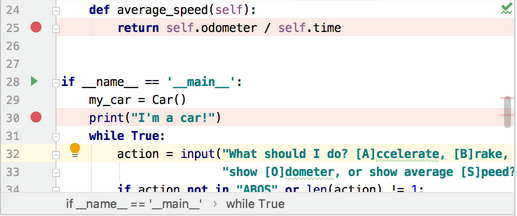
\includegraphics[scale = 0.4]{1}

Znacemo da je Breakpoint uspesno postavljen pojavom crvenog kruzica. Prilikom pokretanja main funkcije naseg programa mozemo izabrati opciju Debug, ovo ce otvoriti \emph{Debug tool window} u kome mozemo pokrenuti nas python kod I gde cemo dobijati sve informacije o izvrsavanju. Informacije koje dobijamo mogu sadrzati poruke o greskama, ne uhvacene izuzeteke, vrednosti promenljivih (u svom zasebnom prozoru) I druge. PyCharm se automatski zaustavlja ukoliko naidje na izuzetak koji nije uhvacen inace se zaustavlja na lokaciji prvog breakpoint-a. Ukoliko program ima vise niti dobicemo posebne prozore za svaku od njih.
\subsection{Detaljno debagovanje}
Sta ako zelimo da posmatramo izvrsavanje naseg koda korak po korak? Da li ovo znaci da moramo postaviti breakpoint u svakoj liniji? Odgovor je ne, PyCharm debugger poseduje , u svom Debug tool window, takozvani \emph{Stepping toolbar}.

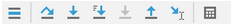
\includegraphics[scale = 0.6]{2}

Cesto koriscene opcije koje su nam na raspolaganju su:
\begin{itemize}
\item  Step Over
\item  Step Into
\item Step Into My Code
\end{itemize}
Step Over jednostavno prelazi na sledecu liniju koda (linija na kojoj se trenutno nalazimo bice osencena u editoru). Step Into opcija ce nas voditi kroz biblioteke I funkcije koje koristimo kada na njih naidjemo
\begin{lstlisting}[language = Python, caption={Primer neki}]
 x = random.nextInt();
 y = f(x);
\end{lstlisting} 
 ovaj kod ce nas odvesti u biblioteku Random ako na ovoj liniji koristimo opciju Step Into tj u definiciju funkcije f, ovo cesto ne zelimo pa koristimo opciju Step Into My Code koja ce nas zadrzati u nasem kodu. 
\subsection{Posmatranja (Watches)}
PyCharm nam omogucava da posmatramo promenljive kroz izvrsavanje naseg programa . U tabu debagera \emph{Variables} se nalaze sve promenljive koje postoje I koje su vidljive u trenutnom stanju izvrsavanja I na trenutnoj lokaciji u kodu  kao I njihov tip I vrednost. Ako klinknemo na \emph {plus} u gornjem levom uglu dobijamo opciju da dodamo bilo koju promenljivu I ona ce biti pracena uvek bez obzira na to gde se ona nalazi , da li je trenutno vidljiva I da li je uopste definisana.
\subsection{Inline Debugger}
Jedna od opcija koju nam pruza PyCharm jeste da klikom na Break point odmah dobijamo informacije o nasim promenljivima I objektima odmah u editoru u vidu komentara. Ova opcija je podrazumevana I mozem se promeniti u Debug Tool window-u.


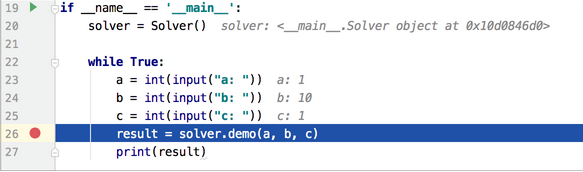
\includegraphics[scale = 0.4]{3}
\subsection{Evaluacija izraza}
Poslednja opcija koja se nalazi na Stepping Toolbar-u je opcija za evaluaciju izraza. Ovo opcija nam omogucava da izracunamo vrednost neke promenljive  koja nam je trenutno u opsegu ili nekog izraza. Pitanje koje se postavlja je zasto bi ovo koristili jer isto mozemo dobiti koriscenjem Posmatranja. Ovo je tacno ali evaluacijom mozemo uraditi nesto sto Posmatranje ne moze a to je da postavimo vrednost nekoj promenljivoj. Ovo je jako korisno jer mozemo testirati nas kod za neke kriticne vrednosti tako sto cemo na `vestack` nacin da dodeljujemo vrednosti promenljivima koje ce nas dovesti do tog kriticnog stanja.

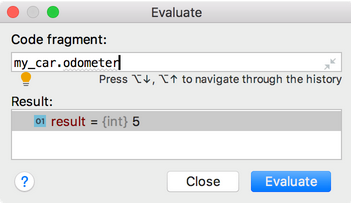
\includegraphics[scale = 0.4]{4}
\section{Zaključak}
\label{sec:zakljucak}

Ovde pišem zaključak. 


\addcontentsline{toc}{section}{Literatura}
\appendix
\bibliography{seminarski} 
\bibliographystyle{plain}

\appendix
\section{Dodatak}
Ovde pišem dodatne stvari, ukoliko za time ima potrebe.


\end{document}
